% DPF 09 talk on strangeness in nucleon

\documentclass[10pt]{beamer}
\usepackage{amsmath}
\usefonttheme{professionalfonts} % using non standard fonts for beamer
\usefonttheme{serif} % default family is serif\
\usepackage{mathtools}
%\documentclass[12pt]{beamerthemeSam.sty}
\usepackage{epsf}
%\usepackage{pstricks}
%\usepackage[orientation=portrait,size=A4]{beamerposter}
\geometry{paperwidth=160mm,paperheight=120mm}
%DT favorite definitions
\def\LL{\left\langle}	% left angle bracket
\def\RR{\right\rangle}	% right angle bracket
\def\LP{\left(}		% left parenthesis
\def\RP{\right)}	% right parenthesis
\def\LB{\left\{}	% left curly bracket
\def\RB{\right\}}	% right curly bracket
\def\PAR#1#2{ {{\partial #1}\over{\partial #2}} }
\def\PARTWO#1#2{ {{\partial^2 #1}\over{\partial #2}^2} }
\def\PARTWOMIX#1#2#3{ {{\partial^2 #1}\over{\partial #2 \partial #3}} }

\def\rightpartial{{\overrightarrow\partial}}
\def\leftpartial{{\overleftarrow\partial}}
\def\diffpartial{\buildrel\leftrightarrow\over\partial}

\def\BI{\begin{itemize}}
\def\EI{\end{itemize}}
\def\BE{\begin{displaymath}}
\def\EE{\end{displaymath}}
\def\BEA{\begin{eqnarray*}}
\def\EEA{\end{eqnarray*}}
\def\BNEA{\begin{eqnarray}}
\def\ENEA{\end{eqnarray}}
\def\EL{\nonumber\\}


\newcommand{\map}[1]{\frame{\frametitle{\textbf{Course map}}
\centerline{\includegraphics[height=0.86\paperheight]{../../map/#1.png}}}}
\newcommand{\wmap}[1]{\frame{\frametitle{\textbf{Course map}}
\centerline{\includegraphics[width=0.96\paperwidth]{../../map/#1.png}}}}

\newcommand{\etal}{{\it et al.}}
\newcommand{\gbeta}{6/g^2}
\newcommand{\la}[1]{\label{#1}}
\newcommand{\ie}{{\em i.e.\ }}
\newcommand{\eg}{{\em e.\,g.\ }}
\newcommand{\cf}{cf.\ }
\newcommand{\etc}{etc.\ }
\newcommand{\atantwo}{{\rm atan2}}
\newcommand{\Tr}{{\rm Tr}}
\newcommand{\dt}{\Delta t}
\newcommand{\op}{{\cal O}}
\newcommand{\msbar}{{\overline{\rm MS}}}
\def\chpt{\raise0.4ex\hbox{$\chi$}PT}
\def\schpt{S\raise0.4ex\hbox{$\chi$}PT}
\def\MeV{{\rm Me\!V}}
\def\GeV{{\rm Ge\!V}}

%AB: my color definitions
%\definecolor{mygarnet}{rgb}{0.445,0.184,0.215}
%\definecolor{mygold}{rgb}{0.848,0.848,0.098}
%\definecolor{myg2g}{rgb}{0.647,0.316,0.157}
\definecolor{abtitlecolor}{rgb}{0.0,0.255,0.494}
\definecolor{absecondarycolor}{rgb}{0.0,0.416,0.804}
\definecolor{abprimarycolor}{rgb}{1.0,0.686,0.0}
\definecolor{Red}           {cmyk}{0,1,1,0}
\definecolor{Grey}           {cmyk}{.7,.7,.7,0}
\definecolor{Lg}           {cmyk}{.4,.4,.4,0}
\definecolor{Blue}          {cmyk}{1,1,0,0}
\definecolor{Green}         {cmyk}{1,0,1,0}
\definecolor{Brown}         {cmyk}{0,0.81,1,0.60}
\definecolor{Black}         {cmyk}{0,0,0,1}

\usetheme{Madrid}


%AB: redefinition of beamer colors
%\setbeamercolor{palette tertiary}{fg=white,bg=mygarnet}
%\setbeamercolor{palette secondary}{fg=white,bg=myg2g}
%\setbeamercolor{palette primary}{fg=black,bg=mygold}
\setbeamercolor{title}{fg=abtitlecolor}
\setbeamercolor{frametitle}{fg=abtitlecolor}
\setbeamercolor{palette tertiary}{fg=white,bg=abtitlecolor}
\setbeamercolor{palette secondary}{fg=white,bg=absecondarycolor}
\setbeamercolor{palette primary}{fg=black,bg=abprimarycolor}
\setbeamercolor{structure}{fg=abtitlecolor}

\setbeamerfont{section in toc}{series=\bfseries}

%AB: remove navigation icons
\beamertemplatenavigationsymbolsempty
\title{
  \textbf {Rotational motion}\\
%\centerline{}
%\centering
%\vspace{-0.0in}
%\includegraphics[width=0.3\textwidth]{propvalues_0093.pdf}
%\vspace{-0.3in}\\
%\label{intrograph}
}

\author[W. Freeman] {Physics 211\\Syracuse University, Physics 211 Spring 2015\\Walter Freeman}

\date{\today}

\begin{document}

\frame{\titlepage}

\frame{\frametitle{\textbf{Announcements}}
\BI
\item{Next homework due next Wednesday}
\item{No office hours today or Friday (I'm traveling)}
\item{Extended office hours: next Monday, 2:30-6:30 (for homework help)}
\item{Due to exam + family illness over the weekend I am very behind on answering mail; I'm sorry!}
\EI
}

\frame{\frametitle{\textbf{Rotational motion}}
  \BI
\item{Everything you've learned about linear motion has a rotational equivalent}
  \BI
\item{Position, velocity, acceleration $\leftrightarrow$ angle, angular velocity, angular acceleration}
\item{Kinematics for coordinates  $\leftrightarrow$ kinematics for angles}
\item{Newton's second law $\leftrightarrow$ Newton's law for rotation}
\item{Force  $\leftrightarrow$ torque}
\item{Mass  $\leftrightarrow$ moment of inertia}
\item{... and others}
  \EI
  \EI
}

\frame{\frametitle{\textbf{Rotational motion}}
  \BI
\item{You already understand angular position, velocity, and acceleration $\rightarrow$ angular kinematics}
\item{You already understand angular momentum ($L=I\omega$, conserved if no external torques)}
\item{We talked about moment of inertia: $I=\lambda mr^2$, where $\lambda$ is some fraction depending on shape}
\pause
\item{\color{Blue}New topic: Newton's second law for rotation}
  \EI
\bigskip

\Huge
\centerline{$\tau = I \alpha$}

\Large\bigskip

\color{Red}
$\rightarrow$ Torques make things have angular acceleration
\BI
\item{What is torque?}
\item{How do we calculate it?}
\EI
}


\frame{\frametitle{\textbf{What corresponds to Newton's second law?}}
  \Large
  \centerline{The key idea in translational motion is Newton's second law $\vec F = m \vec a$.}


  \bigskip
  \bigskip

  \pause

  \centerline{What is the corresponding idea for rotational motion?}

\bigskip
\bigskip

  \BI
\item{Angular acceleration $\alpha$ corresponds to $\vec a$}
\item{The rotational analogue of force is called {\bf \color{Red} torque}}
\item{The rotational analogue of mass is called {\bf \color{Red} moment of inertia}}
  \EI
  \bigskip
  \bigskip

  \pause

  \centerline{Let's look at each of those in turn.}

}

\frame{\frametitle{\textbf{Torque}}
  \Large
  \centerline{Torque ($\tau$) is the rotational analogue of force: ``rotational push or pull''}

  \BI
  \large
\item{Forces applied to an object result in torques: ``push on something to turn it''}
\item{The size of the torque depends on three things:}
  \pause
\item{The size of the force}
  \BI
\item{Push harder to exert more torque -- that's easy!}
  \EI
  \pause
\item{The distance from the force to the pivot point}
  \BI
\item{The further from the pivot to the point of force, the greater the torque}
\item{This is why the door handle is on the outside of the door...}
  \EI
\item{The angle at which the force is applied}
  \BI
\item{Only forces ``in the direction of rotation'' make something turn}
\item{The torque depends only on the {\it component of the force perpendicular to the radius}}
  \EI
  \EI
}
\frame{\frametitle{\textbf{Computing torque}}
  \centerline{\Huge $\tau = F_\perp r$}
\begin{center}
\Large Torque is equal to the distance from the pivot, \\times the perpendicular component of the force
\end{center}


\bigskip
  \centerline{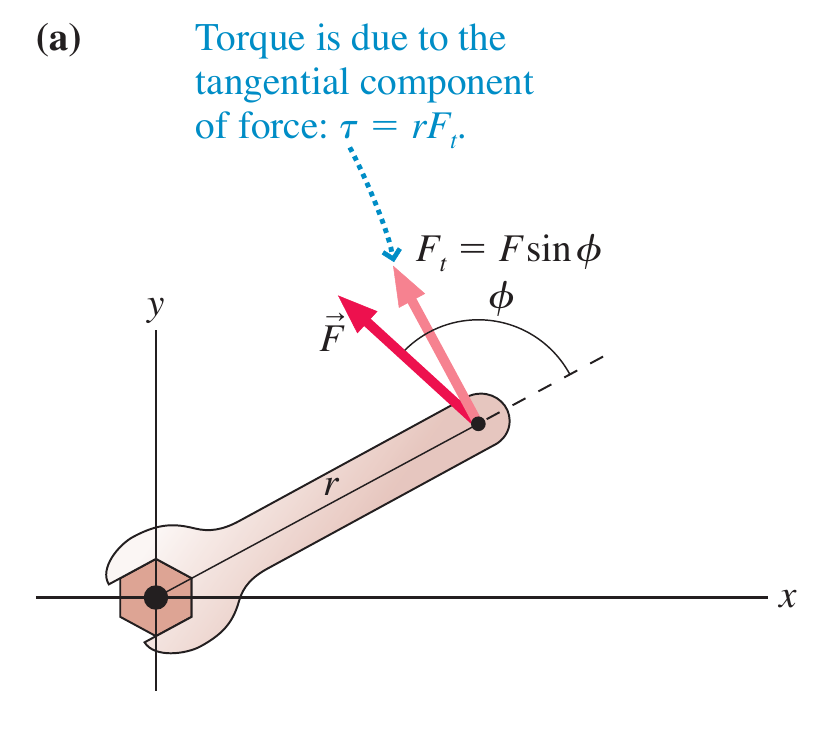
\includegraphics[width=0.3\textwidth]{torque1.png}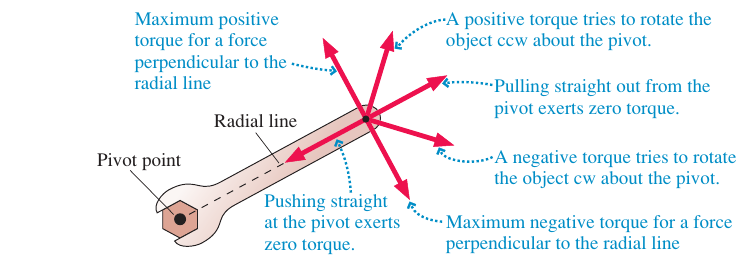
\includegraphics[width=0.6\textwidth]{torque2.png}}

\bigskip

  \centerline{Note that torque has a sign, just like angular velocity: CCW is positive; CW is negative.}
}

\frame{\frametitle{\textbf{Computing torque}}
\BI
\item{We can think of the torque in any other equivalent way; there is another one that's often useful}
\item{The previous way: {\bf ``The radius vector, times the component of force perpendicular to it''}}
\item{The alternative: {\bf ``The force vector, times the component of the radius perpendicular to it''}}
\EI
\centerline{\large{Here's the figure from the text:}}
\centerline{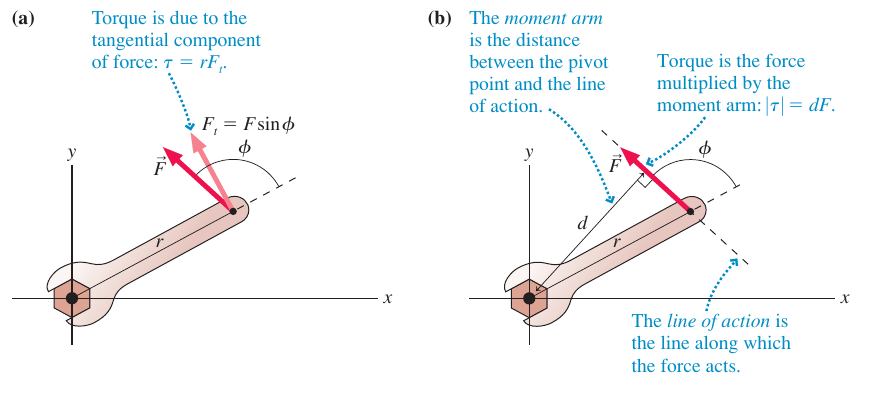
\includegraphics[width=0.6\textwidth]{momentarm.png}}
\bigskip
\centerline{I'll draw a clearer version on the document camera}
}


\frame{\frametitle{\textbf{Important notes about torque}}
  \centerline{\Large These are very important: note them somewhere for later reference!}
  \bigskip
  \bigskip
  \BI
\item{Torques are in reference to a {\bf particular pivot}}
\item{This is different from force; if you're talking about torque, you {\it must} say what axis it's measured around}
\item{Torque now depends on the {\it location} of forces, not just their size}
\BI
\item{Your force diagrams now need to show the place where forces act!}
\item{Weight acts at the center of mass (``the middle''); we'll see what that means later}
\item{A saimple force diagram might look like this:}
  
  \bigskip
  
  \centerline{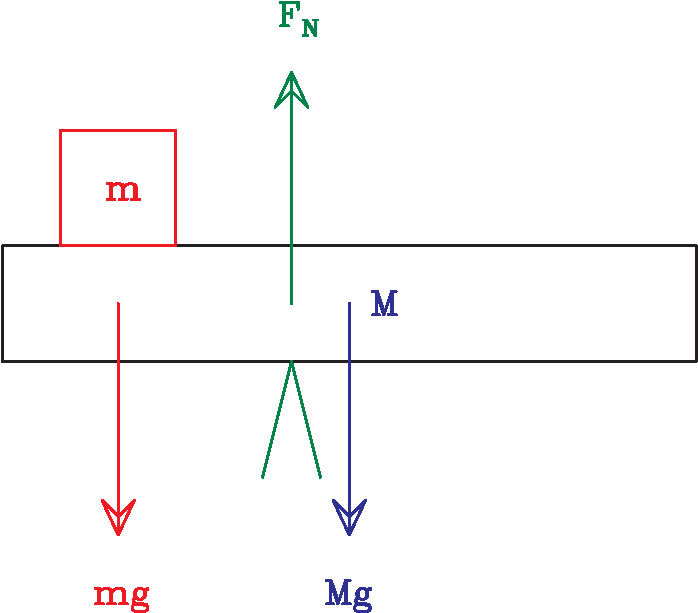
\includegraphics[width=0.3\textwidth]{diag-crop.pdf}}
  \EI
\EI
  }

\frame{\frametitle{\textbf{What about the mass analogue?}}
  \centerline{\Huge $\vec F = m \vec a$}

\medskip

  \centerline{\Huge $\tau =\, ? \alpha$}

  \bigskip
  \bigskip
  \bigskip

  \centerline{\Large Mass tells you how hard it is to give something a (linear) acceleration.}
  \centerline{\Large What determines how hard something is to turn?}
  
  \bigskip
  \bigskip
  \bigskip

\centerline{\Large We can already look at situations where $\tau=\alpha=0$: ``static equilibrium''}
}

\frame{\frametitle{\textbf{Moment of inertia}}
  \centerline{\Large The analogue of mass is called ``moment of inertia'' (letter $I$)}
  
  \BI
  \large
\item{More massive things are harder to turn, but that's only part of it}
\item{The mass {\it distribution} matters, too}
\item{The further the mass is from the center, the harder it will be to turn}
\item{The moment of inertia depends on the {\it average squared distance from the center}}
    \BI
  \item{\color{Lg}I state this without proof here; if you're interested in why, come see me!}
    \EI
  \EI

  \bigskip\pause

  \centerline{\Large $I=MR^2$}

\bigskip
\bigskip
\bigskip

  \centerline{\large (if all the mass is the same distance from the center)}
  \centerline{\large (our demo rods; hoops; rings; bike wheels)} 
}

\frame{\frametitle{\textbf{Moment of inertia, other things}}
  \centerline{\Large What about the moment of inertia of other objects?}
  \centerline{\large Requires calculus in general; here are some common ones} 
  \centerline{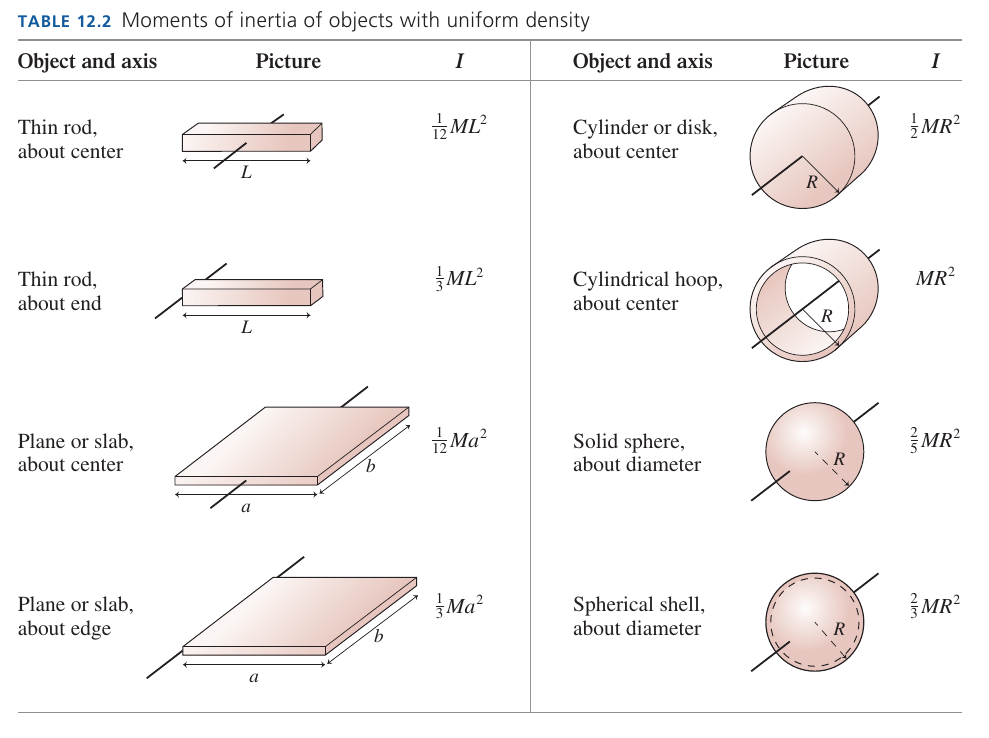
\includegraphics[width=0.7\textwidth]{moment-table.png}}
  }

  \frame{\frametitle{\textbf{Putting it together: Newton's law for rotation}}
    \centerline{
  \begin{tabular}{| c | c |}
    \hline
    Translation & Rotation \\
    \hline
    \hline
    \hline
    Force $\vec F$ & Torque: $\tau=F_\perp r$ \\
    \hline
    Mass $m$ & Moment of Inertia: $I = \lambda MR^2$ \\
    \hline
    Acceleration $\vec a$ & Angular acceleration $\alpha$ \\
    \hline
    \hline
    $\vec F = m \vec a$ & $\tau = I \alpha$ \\
    \hline
  \end{tabular}
}

\bigskip
\bigskip
\bigskip

\centerline{\Large This last line can be thought of as ``Newton's second law for rotation''.}
\bigskip
\bigskip
\bigskip
\centerline{\large Torques give things angular acceleration, just like forces make things accelerate:}
\bigskip
\centerline{\Huge $\tau = I \alpha$}
}

\frame{\frametitle{\textbf{Drawing diagrams: torque problems}}
\Large
\BI
\item{Now you need to draw the position at which every force acts}
\item{Pick a pivot; label it}
\item{Remember, the torque from each force is either...}
\BI
\item{$F_\perp r$ (most useful)}
\item{$F r_\perp$ (sometimes useful)}
\item{$F r \sin \theta$ ($\theta$ is angle between vectors)}
\item{Direction of torques matters!}
\EI
\EI
}

\frame{\frametitle{\textbf{Statics problems}}
\Large
\BI
\item{Often we know $\alpha = \vec a = 0$}
\item{This tells us that the net torque (about {\it any} pivot) and the net force are both zero}
\item{Usually this is because an object isn't moving, but sometimes it's moving at a constant rate (tomorrow's recitation problem)}
\item{Plan of attack:}
\BI
\item{Compute the torque about any point and set it to zero}
\item{Choose a pivot conveniently at the location of a force we don't care about}
\item{If needed, also write $\sum \vec F = 0$}
\EI
\EI
}

\frame{\frametitle{\textbf{Statics problems: a sample}}
\large
\BI
\item{What is the weight of the bar?}
\pause
\item{How does the force needed to support it depend on the angle of the force?}
\pause
\item{How does the force needed to support it depend on the angle of the bar?}
\pause
\item{What if I hang weights from it?}
\EI
}


\end{document}
